
\documentclass[preprint,12pt,a4]{standalone}
\usepackage{geometry}   % my added package "geometry"
\geometry{letterpaper,tmargin=1in,bmargin=1in,lmargin=2.5cm,rmargin=2.5cm}
\usepackage{tikz}
\usetikzlibrary{calc,patterns,arrows.meta,shapes.arrows,intersections,positioning}
\usetikzlibrary{decorations.pathmorphing,backgrounds,fit,petri}
\usepackage{standalone}
\begin{document}
	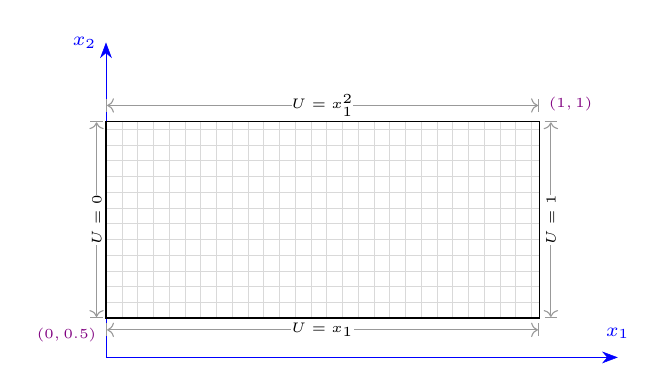
\begin{tikzpicture} [{place/.style={rectangle,draw=blue!50,fill=blue!20,ultra thin,inner sep=0.8mm}},{place2/.style={circle,draw=black!50,ultra thin,inner sep=0.8mm}},{linest/.style={color=gray,ultra thin}}]
	%%coordinates of corners of Beam
	\coordinate (A) at (0.0,0.0);
	\coordinate (B) at (5.5,0.0);
	\coordinate (D) at ($(A)+(0.0,2.5)$);
	\coordinate (C) at ($(B)+(D)$);
	%%axes
	\draw [{Stealth[length=2mm]}-{Stealth[length=2mm]}, help lines,blue] ($(B)+(1,-0.5)$) -- (0,-0.5) -- ($(D)+(0,1)$);
	\node [below,color = blue,font=\scriptsize] at ($(B)+(1,0)$) {$x_1$};
	\node [left,color = blue,font=\scriptsize] at ($(D)+(0,1)$) {$x_2$};
	%%fixed boundary
	%\draw [pattern = crosshatch] ($(A)-(0.1,0.3)$) rectangle ($(D)+(0.0,0.3)$);
	%%mesh
	\draw [line width=0.1pt,gray!30,step=2mm](A) grid (C);
	%%Beam	
	\draw [color=black](A)node[font=\tiny, violet,below left]{$(0,0.5)$} -- (B) -- (C) node[font=\tiny, violet,above right]{$(1,1)$} -- (D) -- cycle;
	%%Concentrate Force Vector
	%\draw [-{Latex[length=2mm]},color=purple, thick] ($(C)+(0.0,1.0)$) -- (C);
	%\node[above,color=purple] at ($(C)+(0.0,1.0)$) {$P$};
	%%B.C
	\draw [|<->|,gray!80]($(A)+(0,-0.15)$) --($(B)+(0,-0.15)$) node[fill=white,midway,inner sep=0.1pt, font=\tiny,text=black] {$U=x_{1}$};
	\draw [|<->|,gray!80]($(B)+(0.15,0.0)$)--($(C)+(0.15,0.0)$) node [fill=white,midway, sloped, font=\tiny, inner sep=0.05pt, text=black] {$U=1$};
	
	\draw [|<->|,gray!80]($(C)+(0,0.2)$) --($(D)+(0,0.2)$) node[fill=white,midway,inner sep=0.01pt, font=\tiny,text=black] {$U=x_{1}^2$};
	\draw [|<->|,gray!80]($(A)+(-0.12,0.0)$)--($(D)+(-0.12,0.0)$) node [fill=white,midway,sloped, font=\tiny, inner sep=0.05pt, text=black] {$U=0$};
	\end{tikzpicture}
\end{document}